\section{Introduction}
\IEEEPARstart{S}{ynthetic} aperture radar (SAR) maps floods through cloud and at night, which makes
Sentinel-1 the workhorse of rapid flood mapping. Deep segmentation networks trained on labelled SAR
scenes now reach high accuracy on standard benchmarks, but a rapid-mapping model is always applied to a
flood it has not seen: a new river, a new landscape, a new season. Errors concentrate where backscatter
is ambiguous---radar shadow and layover in hilly terrain, smooth dry surfaces such as sand and tarmac,
wet soil, and vegetation over water---and which of these a model has learned to handle depends on the
floods it was trained on.

Terrain is the obvious physical prior. Water collects low and close to drainage, and elevation data are
global, free and available before the flood: the Copernicus GLO-30 digital elevation model
(DEM)~\cite{glo30dem} and the height above nearest drainage (HAND) derived from it~\cite{renno2008hand,
nobre2011hand,asfhand}. Physics-informed and physics-guided deep learning offers several ways to inject
such a prior: as an extra input, as a loss that penalizes physically implausible outputs, or as a
post-processing mask. Whether any of them helps on a \emph{new} flood is less clear than it may seem.
Most published comparisons use random or official tile splits of a single dataset, so training and test
tiles share flood events, and the comparison measures how well a model fits a known event rather than
how well it transfers.

This paper evaluates terrain priors where they matter, on flood events the model has not seen. We treat
the flood event as the unit of analysis throughout: we hold out whole events, score every event
separately, and compare model variants with paired statistics over events and over training seeds or
draws. Training on Sen1Floods11~\cite{bonafilia2020sen1floods11} and testing on 79 Copernicus Emergency
Management Service (CEMS) activations from GEOID-Flood~\cite{geoidflood} gives a test set large enough to
detect gains of a few points in intersection over union (IoU); training on subsets of GEOID-Flood's 159
training events shows how the value of terrain changes as more floods are labelled.

\begin{figure*}[t]
\centering
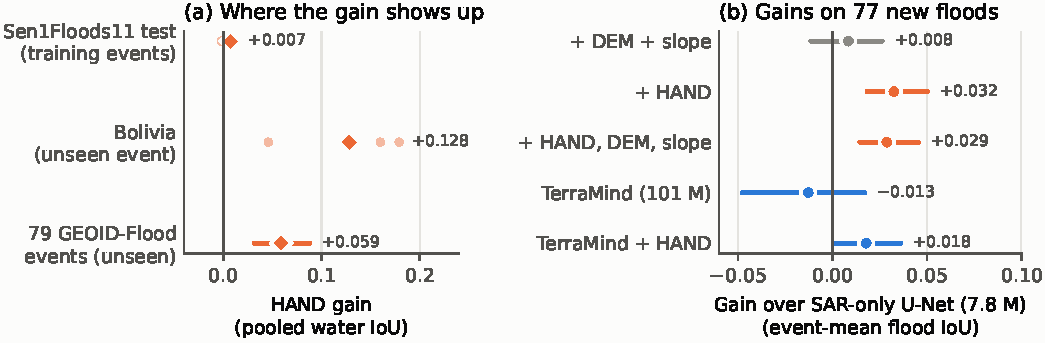
\includegraphics[width=\textwidth]{fig_overview.pdf}
\caption{Models trained on the 11 Sen1Floods11 events. (a) HAND gain in pooled water IoU on Sen1Floods11's
test split (tiles from the training events), its Bolivia hold-out and 79 external GEOID-Flood events (dots:
seeds; diamonds: means; bar: 95\% CI). (b) Gain over the SAR-only U-Net in event-mean flood IoU on 77
GEOID-Flood events (two-way 95\% CIs).}
\label{fig:overview}
\end{figure*}

Three findings stand out (Fig.~\ref{fig:overview}):
\begin{enumerate}
\item \emph{Same-event splits hide the value of terrain.} A U-Net trained on Sen1Floods11 gains almost
nothing from HAND on that dataset's official test split (+0.007 IoU), whose tiles come from the training
events, but +0.128 on its held-out Bolivia event and +0.059 in pooled water IoU over 79 external floods
(+0.061 in mean event IoU, improving 69 of them).
\item \emph{The gain needs correctly located, detailed height above drainage.} In this transfer, elevation
and slope recover only a quarter of it at the event level; shifting HAND by 500\,m in each axis,
blurring it, or swapping in another flood's HAND removes the event-level gain, and a model trained with mismatched HAND gains nothing, so it
is not a side effect of an extra input channel. A permanent-water map recovers none of the flood-extent
gain and, with many training events, teaches the model to look for water only where it already was.
\item \emph{A foundation model does not replace terrain.} HAND helps a fine-tuned 101\,M-parameter
TerraMind~\cite{jakubik2025terramind} about as much as it helps a 7.8\,M-parameter U-Net in event-mean
flood IoU (less for all water), and the small U-Net with HAND beats TerraMind without it.
\end{enumerate}

We also show that HAND as a physics loss or mask does nothing, even when the loss demonstrably enforces its
constraint; that the input gain survives threshold-free scoring, GEOID-Flood's own protocol and resampling
by country, and where it occurs by HAND, slope and land cover; that with 159 GEOID-Flood training events the
flood-extent gain is no longer detectable (a pre-registered test of a steady decline was null), while 500
tiles from all 159 events match all 8,712; and that two pre-registered remedies for HAND's failure cases do
not help. The full pipeline, run outputs and checkpoints are released.
